%! TeX Program = lualatex
%^Tells VimTex to use lualatex.

% preamble {{{1
\documentclass{beamer}

\usepackage{xfrac}
\usepackage{emoji} %emoji
\usepackage{hyperref} %links
\usepackage{xcolor} %colors
\usepackage{tikz} %drawing custom underlines
\usepackage{type1cm} %make fonts scalable
\usepackage{lettrine} %drop caps
\usepackage{lipsum} %blindtext
\usepackage[T1]{fontenc} %set font encoding
\usepackage{adforn} %more ornaments
\usepackage{booktabs} %better tables
\usepackage{pgfplots} %for plots
\usepackage{mathtools} %math symbols
\usepackage[tworuled, algosection]{algorithm2e} %for building psuedocode env
\usepackage{amsmath} %math
\usepackage{amsthm} %theorem envs
\usepackage{amsfonts} %math fonts
\usepackage{mathrsfs} %math script letters
\usepackage[backend=biber]{biblatex} %bibliography
\usepackage{background} %page background
\usepackage{calligra} %calligraphic fonts

%psuedocode env stolen from matt moore (https://ittc.ku.edu/~moore/) {{{2
\newenvironment{pseudocode}
  { \begin{center} \begin{algorithm}[H]
    \SetStartEndCondition{ }{}{}
    \AlgoDontDisplayBlockMarkers
    \SetAlgoNoEnd
    \DontPrintSemicolon
    \SetArgSty{}

    \SetKwFor{Define}{define}{}{}
    \SetKwFor{For}{for}{}{}
    \SetKwFor{While}{while}{}{}
    \SetKwIF{If}{ElseIf}{Else}{if}{}{elif}{else}{}
    \SetKw{Break}{break}
    \SetKw{In}{in}
    \SetKw{Let}{let}
    \SetKw{Return}{return}
    \SetKwComment{Comment}{\texttt{\#} }{}
    \SetCommentSty{textit}
  }
  { \end{algorithm} \end{center} }
  %}}}2

%link stuff {{{2
\definecolor{linkcolor}{rgb}{0,0,0} %links are colorless
\hypersetup{colorlinks,breaklinks,urlcolor=linkcolor,linkcolor=linkcolor,citecolor=linkcolor} %hyperref settings

\renewcommand{\LettrineTextFont}{\rmfamily} % make drop cap text after not smallcaps.
%2}}}

%beamer theming {{{1
\usetheme{Boadilla}
\usecolortheme{seahorse}
\setbeamertemplate{navigation symbols}{}
%1}}}
%1}}}

\begin{document}

%title matter {{{1

\title{Path Finding Star Power \emoji{star-struck}}
\subtitle{An Analysis of the $A^*$ Algorithm}
\author{James Hurd}
\date{\today}

%1}}}

% toc {{{1

\frame{\titlepage}

\begin{frame}{outline}
  \frametitle{Table of Contents \emoji{fountain-pen}}

\tableofcontents

\end{frame}
%1}}}

%object of study {{{1
\section{Object of Study \emoji{books}}
\begin{frame} 
  \frametitle{Object of Study \emoji{books}}
  
  \begin{block}{Definition: $\delta$ Graph}

    A \textbf{$\delta$ graph} is a directed, weighted graph where the cost of each edge is is
    strictly greater than $\delta$ where $\delta$ is a positive real number.

  \end{block}

\end{frame}
%1}}}

% problem at hand {{{1
\section{The Problem at Hand \emoji{thinking-face}} 
\begin{frame} 
  \frametitle{The Problem at Hand \emoji{thinking-face}}

  Give a $\delta$ graph $G$, we would like to find a \textit{minimum-cost} path from some starting
  vertex to a \textit{preferred goal vertex} of $s$.

  \begin{block}{Definition: Preferred Goal Vertex}
  
    Given some vertex $s$ and a set of goal vertices $T$ in a graph $G$, 
    a \textbf{preferred goal vertex} of $s$ is a vertex $t$ in $T$ such that
    the cost of a path from $s$ to $t$ is minimal.

  \end{block}

\end{frame}
%1}}}

% introducing A* {{{1
\section{Introducing\dots $A^*$ \emoji{star}}
\begin{frame} 
  \frametitle{Introducing\dots $A^*$ \emoji{star}}

  \begin{block}{Definition: Admissibility}
  
  We say an algorithm is \textbf{admissible} if it is guaranteed to 
  return a minimum-cost path for \textit{any} $\delta$ graph.
  \end{block}

The $A*$ algorithm is the \textbf{most optimal} algorithm for solving
the minimum-cost paths problem in the sense that it expands
the least amount of vertices possible (given the information it has).

\end{frame}
%1}}}

% eval func {{{1
\section{A Key Ingredient for an Optimal Algorithm \emoji{cook}}
\begin{frame} 
  \frametitle{A Key Ingredient for an Optimal Algorithm \emoji{cook}}

  $A^*$ would like to expand the least amount of vertices possible.

  \begin{block}{Helpful Tool: The Evaluation Function}
    The \textbf{evaluation function $\hat{f}$} helps $A*$ decide which vertex to expand next. For a vertex $v$,
    \begin{equation*}
      \hat{f}(v) = \hat{h}(v) + \hat{g}(v)
    \end{equation*}

    Where $\hat{g}(v)$ is the cost of the path from the starting vertex $s$ to $v$ with the minimum
    cost found so far and $\hat{h}(v)$ is a \textit{heuristic}.
  \end{block}

\end{frame}
%1}}}

% heuristic {{{1
\section{Wait, What's a Heuristic? \emoji{face-with-spiral-eyes}}
\begin{frame} 
  \frametitle{Wait, What's a Heuristic? \emoji{face-with-spiral-eyes}}

  A \textbf{heuristic} is a function that \textit{estimates} a particular
  quantity. In $A*$, our heuristic will often use information from the
  problem domain. $\hat{h}$ must satisfy two constraints for all
  vertices $v$ and $w$:

  \begin{itemize}

    \item $\hat{h}(v) \leq h(v)$
    \item $\hat{h}(v) \leq \hat{h}(v,w) + \hat{h}(w)$ (consistency)

  \end{itemize}
  
  Some example choices of $\hat{h}$:
  \begin{itemize}
    \item $\hat{h}(v) = 0$ for all $v$
    \item ``Taylor Swift Distance''
  \end{itemize}

\end{frame}
%1}}}

% algo {{{1
\section{The \textit{Star} of the Show \emoji{woman-cartwheeling}}
\begin{frame} 
  \frametitle{The \textit{Star} of the Show \emoji{woman-cartwheeling}}
  

  \begin{pseudocode} 
    \footnotesize
    \Define{\texttt{A*}$(s, T)$}{ 
      Mark $s$ as ``open'' and calculate $\hat f(s)$ \;

      \Let $pred=[]$\;
      
      \While{True}{
        \Let $n$ = ``open'' vertex whose value of $\hat{f}$ is minimal.
        Resolve ties arbitrarily but always in favor of a vertices in $T$. \;
        Mark $n$ as ``closed''.\;
        \If{$n\in T$}{
          Reconstruct an optimal path using $pred$ starting with
          $n$ and terminate.
        }
        \Let $succs = \Gamma(n)$ \;
        \For{$v\in succs$} {

          $pred[v]= n$ \;
          
            Calculate $\hat{f}(v)$. \;

            \If{$v$ is not marked ``closed'' or $\hat{f}$(v) is smaller than before}{
              
              Mark $v[0]$ as ``open''.\;

            }

          }
      }

    }
  \end{pseudocode} 

\end{frame}
%1}}}

% examples {{{1
\section{$A^*$ in Action \emoji{woman-dancing}}
\begin{frame} 
  
  \begin{center}
    \LARGE
    Let's see some examples of $A^*$ in action! \emoji{woman-dancing}
  \end{center}

\end{frame}
%1}}}

% thanks {{{1
\begin{frame} 
 
  \begin{center}
    \Large{
      Thank you! \emoji{heart}

    Questions?
    
    \vspace{0.5em}

    \fcolorbox{black}{black}{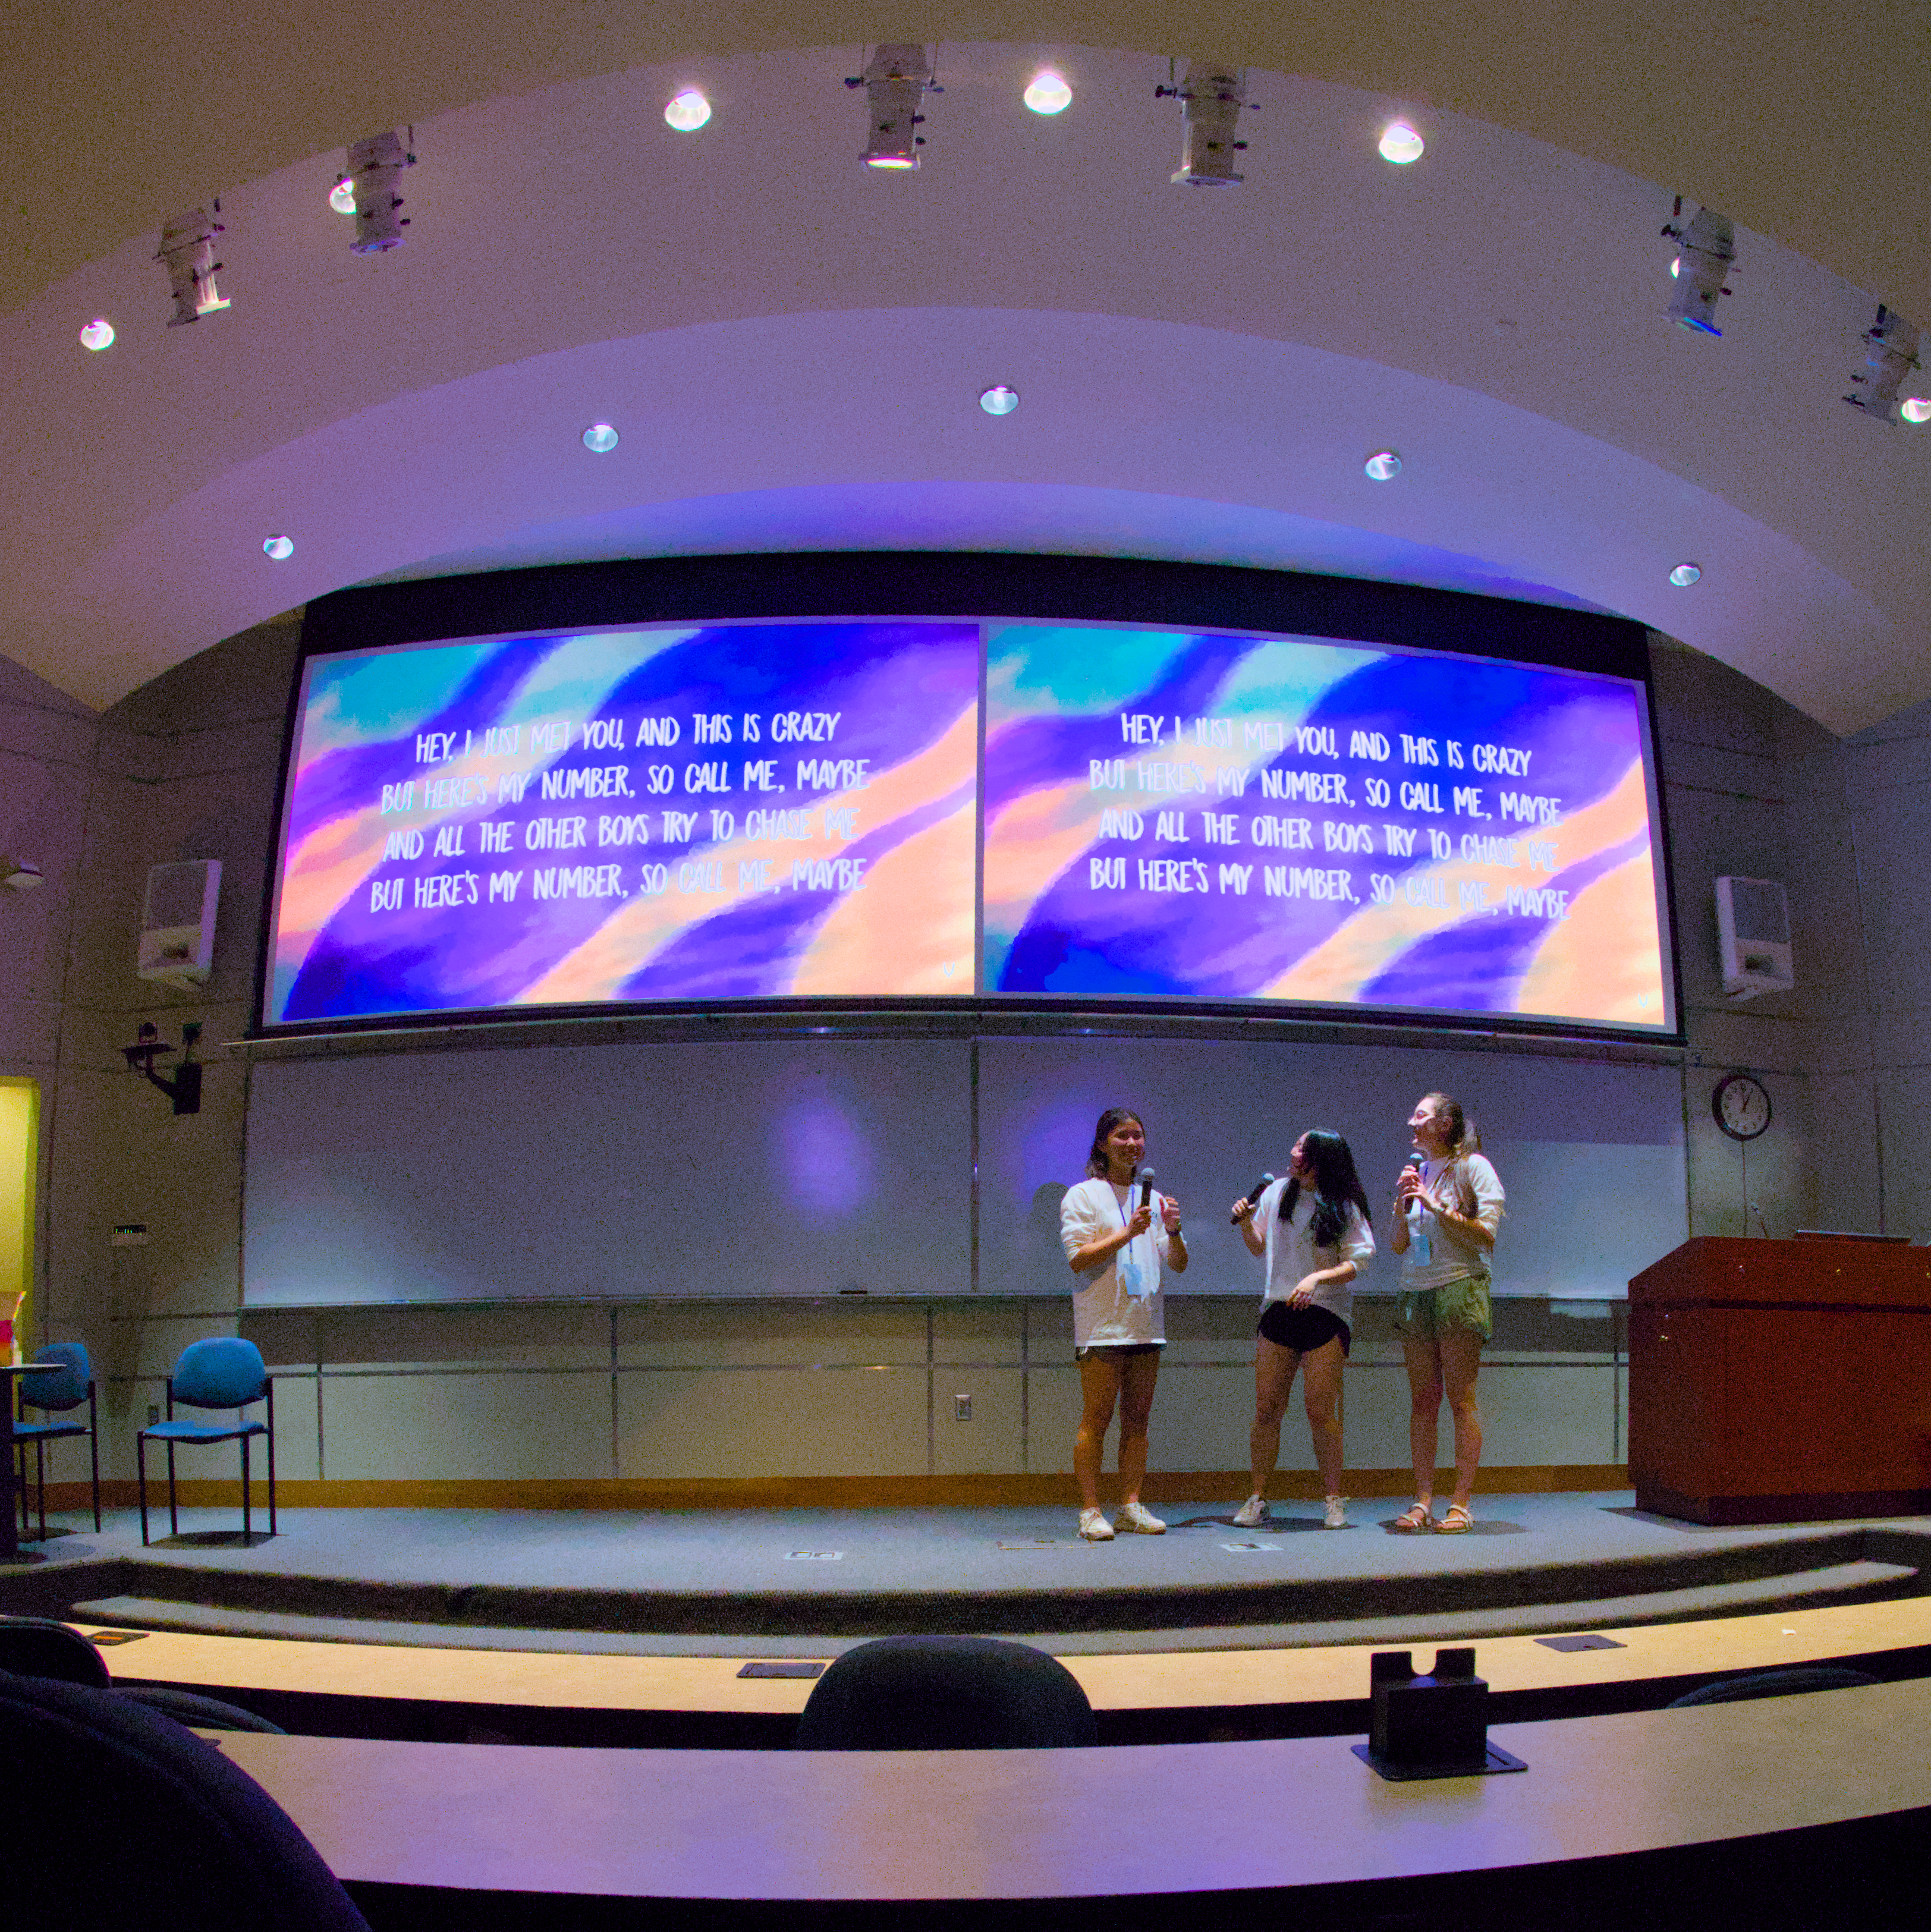
\includegraphics[scale=0.18]{karaoke}}

    \vspace{0.5em}

    \href{mailto:jmh@ku.edu}{\texttt{jmh@ku.edu}}

    \href{https://jameshurd.net/projects/star-power}{\texttt{jameshurd.net/projects/star-power}}

    \hfill{\calligra{fin.}}
  }
  \end{center}

\end{frame}
%1}}}
\end{document}
